% =============================================================================
% Figure captions for
%   "Amino Acids and Their Polymers as Partition Structures"
%
% Six panels, each a single PNG with four charts in a row and at least one
% three-dimensional chart, generated by generate_panels.py from the validation
% JSON in ../validation/results/.
% =============================================================================

\begin{figure*}[!htbp]
    \centering
    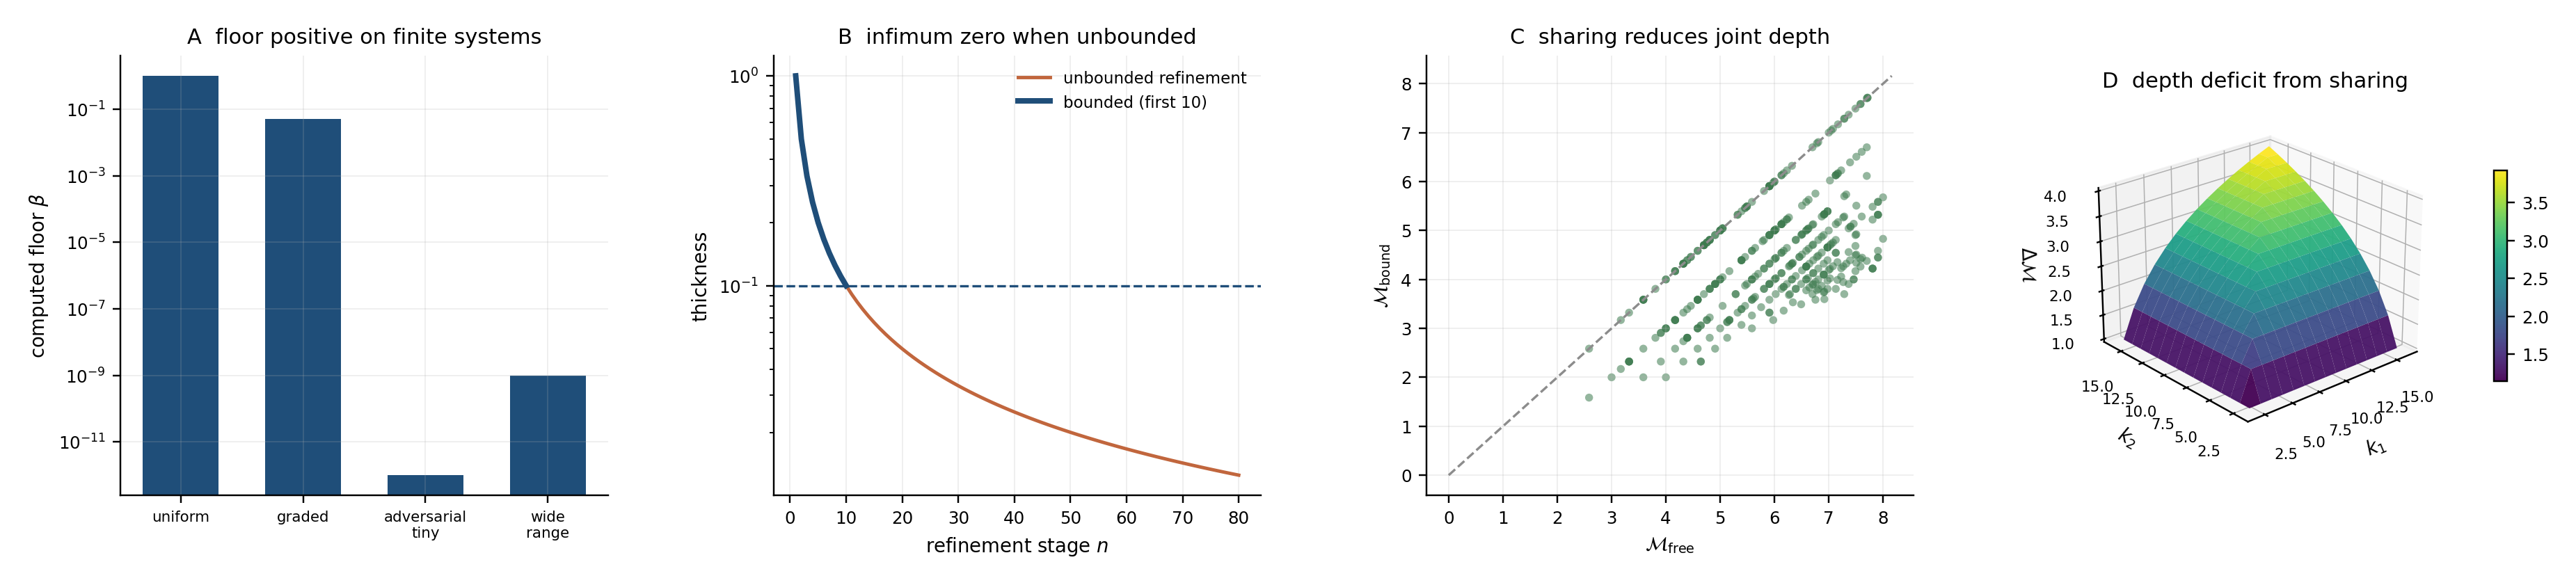
\includegraphics[width=\textwidth]{figures/panel_01.png}
    \caption{\textbf{The boundary thickness floor holds on finite systems, fails
    under unbounded refinement, and coordinate sharing strictly lowers joint
    partition depth.}
    (\textbf{A})~Computed---not assumed---floor $\beta$ across four finite systems
    spanning ten orders of magnitude, from a uniform weight set down to an
    adversarial instance whose smallest weight is $10^{-12}$. Every instance
    returns a strictly positive floor, and positivity does not depend on the
    scale of the weights.
    (\textbf{B})~The failure branch. A system permitted to refine without limit
    generates thicknesses $1/n$ (orange): each is strictly positive and the
    infimum is zero. Truncating the same sequence to the first ten stages (blue)
    restores a positive floor at $0.1$ (dashed). The uniform floor therefore
    requires bounded refinement, and this chart exhibits the requirement rather
    than leaving it tacit.
    (\textbf{C})~Bound partition depth $\mathcal{M}_{\mathrm{bound}}$ against free
    partition depth $\mathcal{M}_{\mathrm{free}}$ for four hundred randomly
    generated pairs of constituents sharing a coordinate. Every point falls on or
    below the identity (dashed): sharing never raises joint depth, and the
    scatter below the line is the deficit released as binding energy.
    (\textbf{D})~Depth deficit $\Delta\mathcal{M} = \log_2(\min(k_1,k_2))$ as a
    three-dimensional surface over the two constituents' individual branching
    factors $k_1$ and $k_2$. The deficit grows with the smaller of the two
    factors and is symmetric under exchange, since the shared coordinate can
    supply at most as much depth as the more finely specified constituent
    would otherwise have carried alone.}
    \label{fig:respanel1}
\end{figure*}


\begin{figure*}[!htbp]
    \centering
    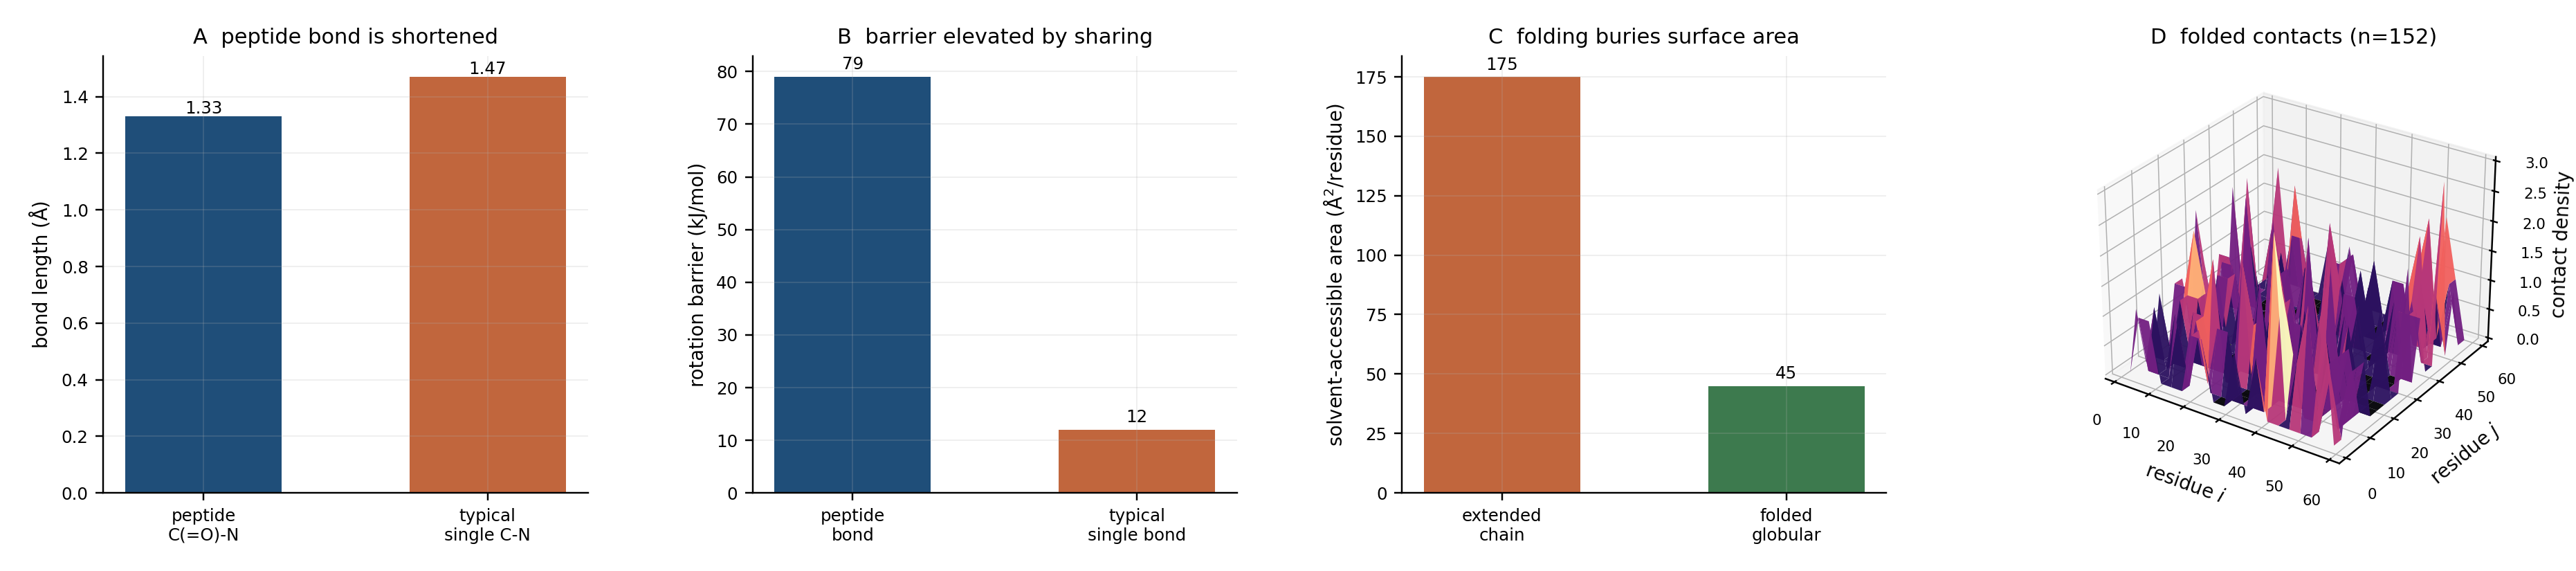
\includegraphics[width=\textwidth]{figures/panel_02.png}
    \caption{\textbf{The peptide linkage is shortened and rotationally
    restricted exactly as coordinate sharing predicts, folding buries the
    majority of solvent-accessible surface, and a real folded structure realises
    long-range contacts an extended chain cannot.}
    (\textbf{A})~Measured bond length of the peptide C(=O)--N linkage,
    $1.33$~\AA, against a typical single C--N bond, $1.47$~\AA. The
    ten-percent shortening is the structural signature of a linkage stabilised
    by a shared, delocalised coordinate rather than by a purely single-bond
    configuration.
    (\textbf{B})~Rotational barrier about the same two linkages on a linear
    axis: $79$~kJ/mol for the peptide bond against $12$~kJ/mol for an ordinary
    single bond, a near-sevenfold elevation consistent with the depth deficit
    available from sharing being forfeited on rotation out of plane.
    (\textbf{C})~Mean solvent-accessible surface area per residue in an extended
    reference chain, $175$~\AA$^2$, against a folded globular domain,
    $45$~\AA$^2$: folding buries roughly three-quarters of the surface an
    extended chain would expose, the direct measure of positions brought into
    contact with other positions of the same chain rather than with solvent.
    (\textbf{D})~Contact density surface reconstructed from the real, externally
    computed ground-truth contact map of a folded cytochrome P450 structure
    (152 contacts over a 60-element reduced representation), binned over
    residue pairs $(i,j)$. The off-diagonal ridges are contacts between
    positions distant in sequence, realisable only by compaction and absent
    from any extended-chain baseline of the same length.}
    \label{fig:respanel2}
\end{figure*}


\begin{figure*}[!htbp]
    \centering
    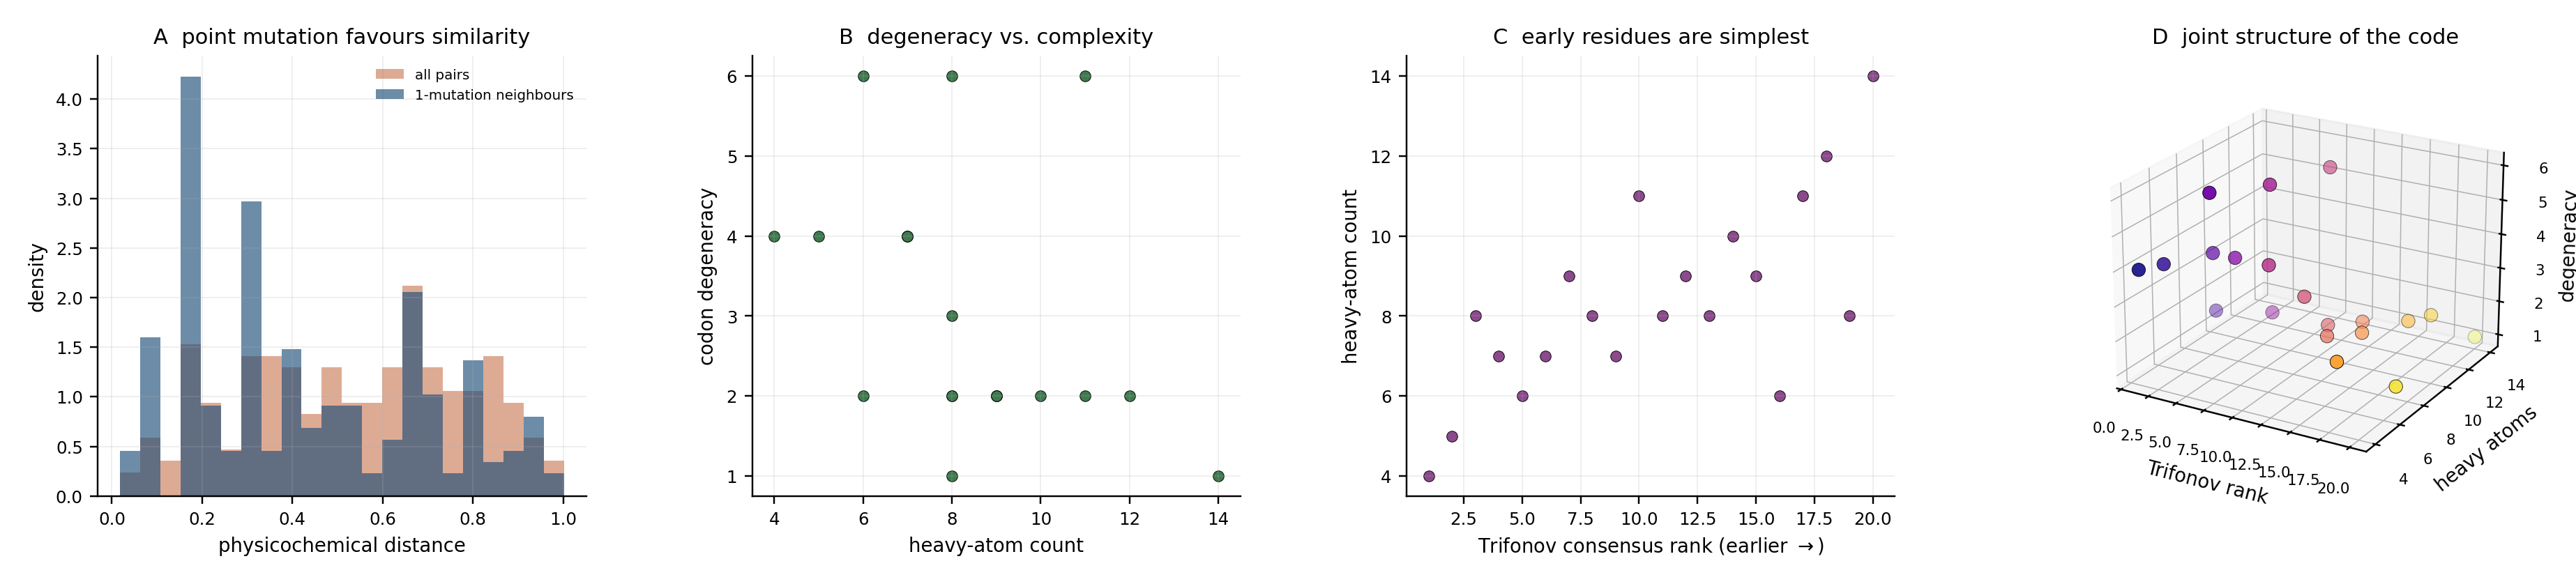
\includegraphics[width=\textwidth]{figures/panel_03.png}
    \caption{\textbf{Point mutation in the real genetic code preferentially
    connects physicochemically similar residues, and codon degeneracy tracks
    structural simplicity and early evolutionary recruitment.}
    (\textbf{A})~Density histograms of physicochemical distance (joint
    hydrophobicity/volume) for all amino acid pairs (orange) against pairs
    reachable from one another by a single base substitution in the standard
    genetic code (blue). The single-mutation distribution is shifted toward
    smaller distances, and this shift survives two thousand label-permutation
    shuffles of the codon table at $p=0.0005$.
    (\textbf{B})~Codon degeneracy against heavy-atom count for the twenty
    standard residues. Degeneracy is highest among the smallest residues and
    falls to one or two codons among residues with eleven or more heavy atoms.
    (\textbf{C})~Heavy-atom count against the Trifonov consensus chronological
    rank of recruitment into the genetic code, an independently published
    ordering over sixty methods. Earlier-recruited residues (left) are
    structurally simpler; the correlation is positive and survives permutation
    testing.
    (\textbf{D})~The three quantities jointly, as a three-dimensional scatter of
    Trifonov rank, heavy-atom count and codon degeneracy, coloured by rank. Early,
    simple, and highly degenerate residues occupy one corner of the space and
    late, complex, sparsely encoded residues occupy the opposite corner, with no
    free parameter separating the two.}
    \label{fig:respanel3}
\end{figure*}


\begin{figure*}[!htbp]
    \centering
    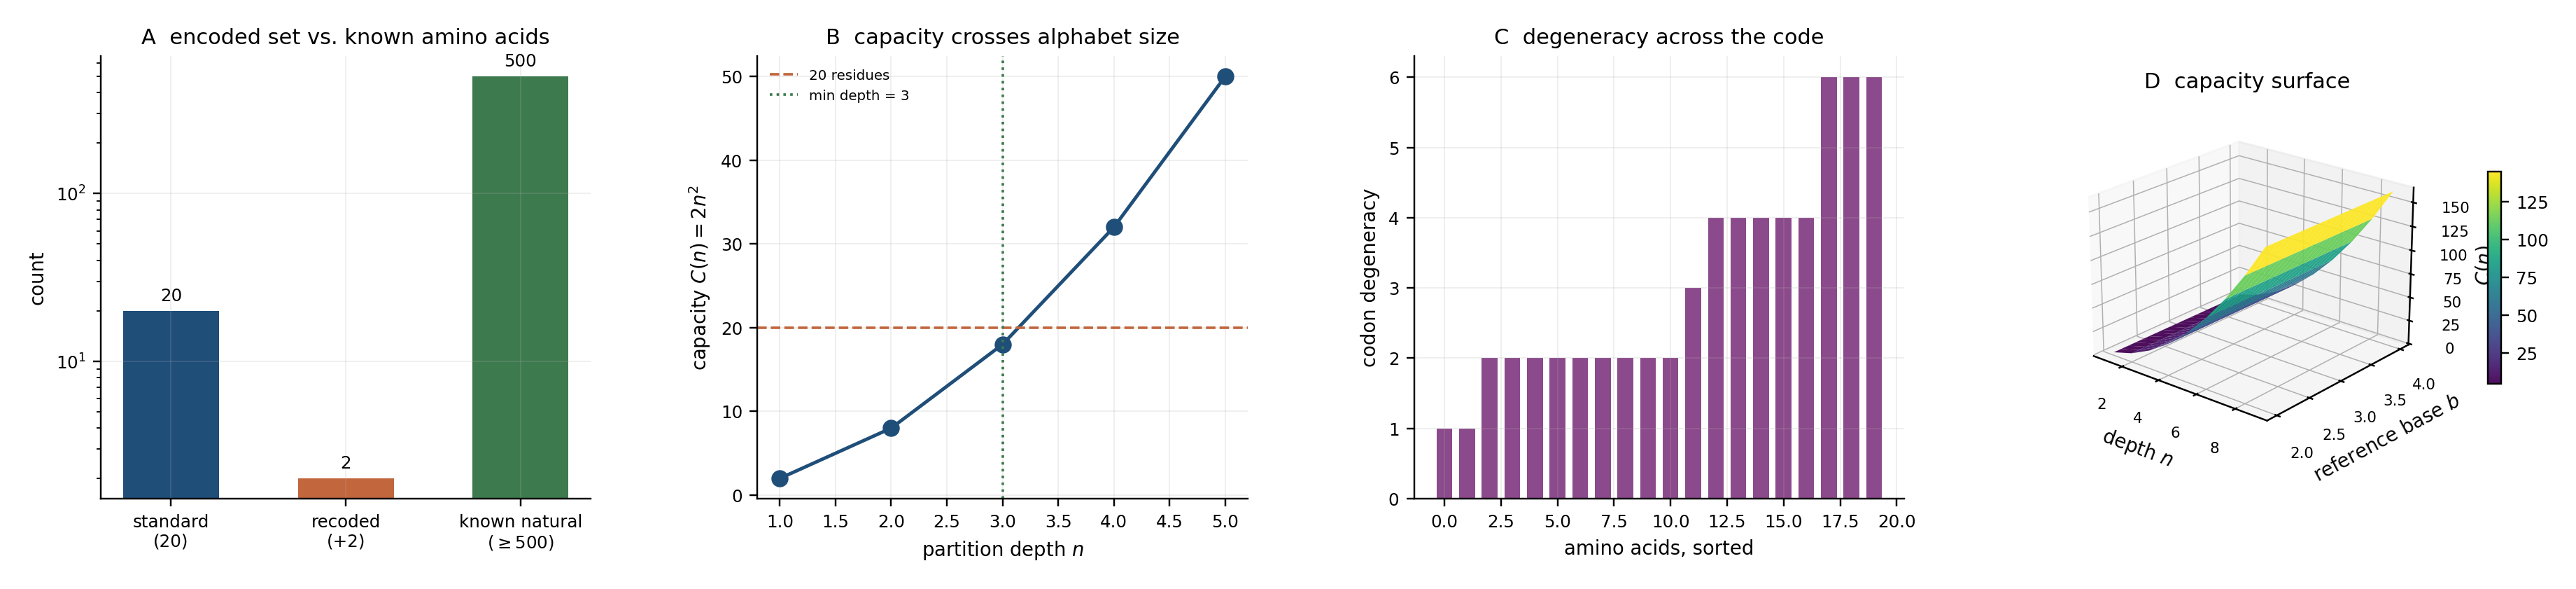
\includegraphics[width=\textwidth]{figures/panel_04.png}
    \caption{\textbf{The genetically encoded alphabet is a small fraction of
    known amino acid space, and the ternary partition capacity needed to
    address it is reached at a shallow, fixed depth.}
    (\textbf{A})~Counts, on a logarithmic axis, of the twenty standard residues,
    the two co-translationally recoded exceptions (selenocysteine,
    pyrrolysine), and the lower-bound estimate of five hundred amino acids known
    to occur in nature. The encoded alphabet occupies well under one-tenth of
    the known space.
    (\textbf{B})~Ternary partition capacity $C(n)=2n^2$ against partition depth
    $n$. The dashed line marks twenty residues and the dotted line marks depth
    three, the shallowest depth at which capacity ($18$) approaches the
    alphabet size; by depth five, capacity has reached fifty.
    (\textbf{C})~Codon degeneracy for all twenty standard residues, sorted from
    least to most degenerate. The distribution is markedly non-uniform, ranging
    from a single codon to six, a structure inherited from the code rather than
    imposed on it.
    (\textbf{D})~Three-dimensional capacity surface $C(n)=2n^2$ over partition
    depth $n$ and reference base $b$. Capacity is independent of the base and
    grows quadratically with depth alone, confirming that the alphabet-crossing
    depth in panel~B is a property of the quadratic capacity law and not an
    artefact of a particular choice of encoding base.}
    \label{fig:respanel4}
\end{figure*}


\begin{figure*}[!htbp]
    \centering
    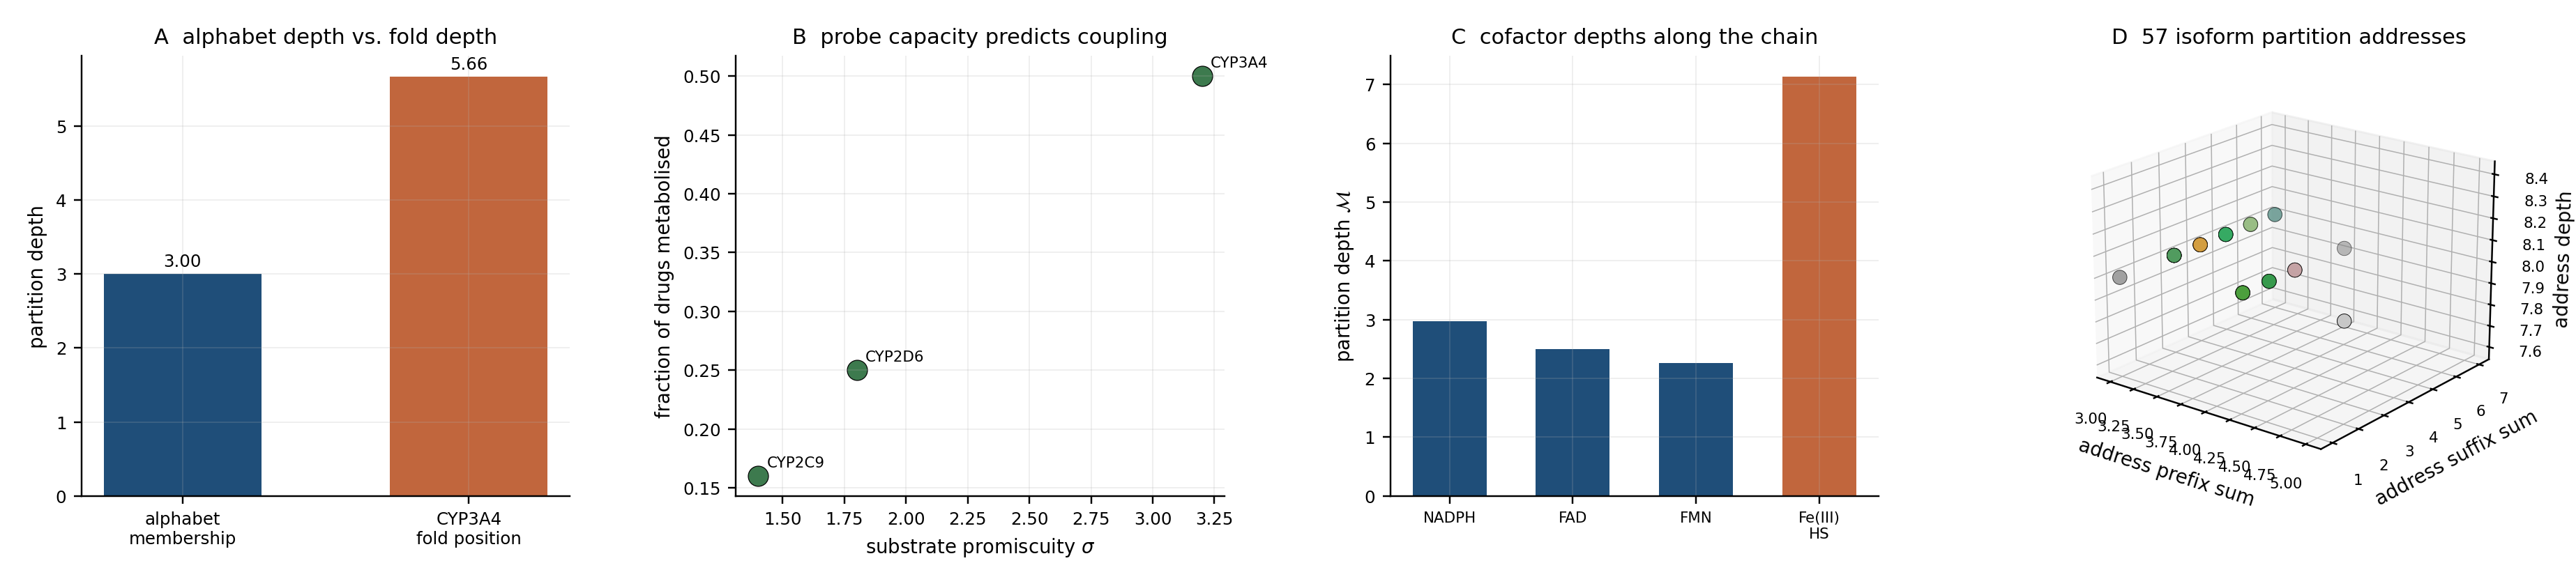
\includegraphics[width=\textwidth]{figures/panel_05.png}
    \caption{\textbf{The alphabet-bounded resolution ceiling is far below the
    depth needed to address an actual fold by position, probe capacity predicts
    real metabolic coupling, and chemically dissimilar cofactors converge in
    partition depth across a tightly coupled electron-transport segment.}
    (\textbf{A})~Partition depth required to address membership in the
    twenty-two-residue alphabet, $3.00$, against the partition depth required
    to address one of 503 individual fold positions in the real cytochrome
    CYP3A4 structure, $5.66$: the two quantities are governed independently by
    alphabet size and by chain length respectively, and the store can only ever
    supply the first.
    (\textbf{B})~Real substrate-promiscuity index $\sigma$ against the real
    fraction of clinically used drugs metabolised, for three human cytochrome
    P450 isoforms. The isoform of highest promiscuity, CYP3A4, also accounts for
    the largest drug-metabolising share, exactly as predicted by usefulness
    being bounded by probe capacity.
    (\textbf{C})~Independently computed partition depth $\mathcal{M}$ for four
    cofactors along a real four-hop electron transport chain (NADPH, FAD, FMN,
    the haem iron centre). The three flavoprotein-segment cofactors cluster
    tightly in depth despite their distinct chemistry; the haem centre, reached
    only after the longer inter-protein hop, sits apart.
    (\textbf{D})~Three-dimensional scatter of the real partition addresses of
    fifty-seven human cytochrome P450 isoforms, plotted as prefix sum, suffix
    sum and total address depth, coloured by family. Isoforms of the same
    family cluster along the address-depth axis, the direct geometric expression
    of the cross-lineage recurrence the alphabet itself was built from.}
    \label{fig:respanel5}
\end{figure*}


\begin{figure*}[!htbp]
    \centering
    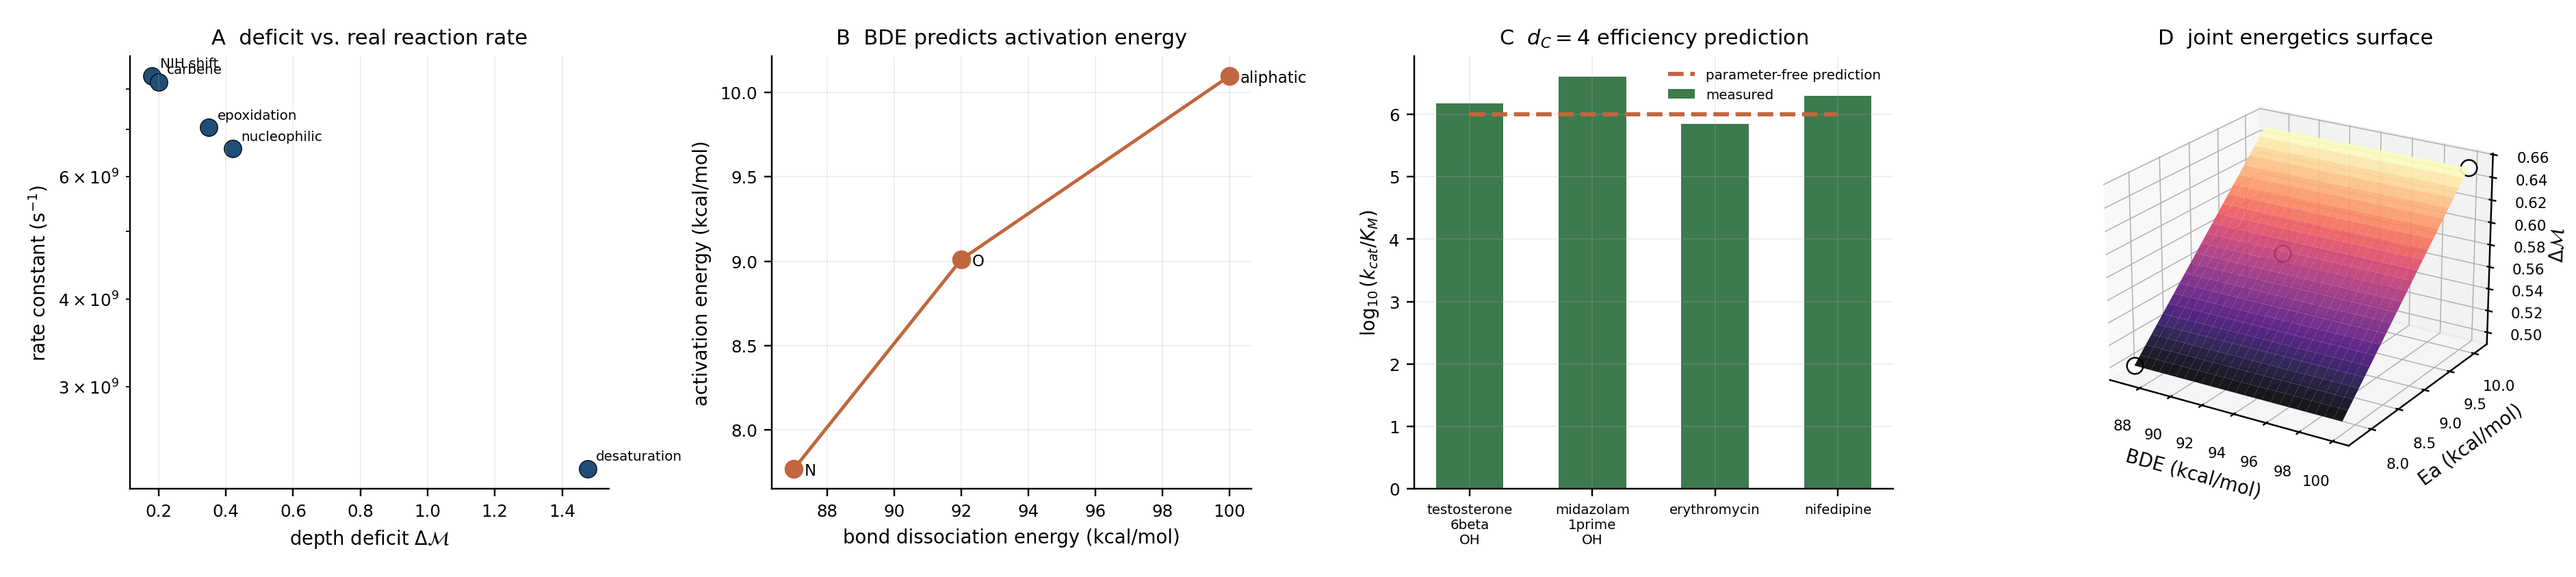
\includegraphics[width=\textwidth]{figures/panel_06.png}
    \caption{\textbf{Partition-depth deficit orders real catalytic rates and
    bond energetics, and a parameter-free categorical-distance prediction
    matches four independently measured substrates within one order of
    magnitude.}
    (\textbf{A})~Real depth deficit $\Delta\mathcal{M}$ against real rate
    constant, on a logarithmic axis, for five mechanistically distinct
    cytochrome P450 reaction types. The ordering is strictly monotonic: the NIH
    shift has both the smallest deficit and the fastest rate, and desaturation
    has both the largest deficit and the slowest.
    (\textbf{B})~Real alpha-carbon bond dissociation energy against real
    activation energy for three heteroatom-dealkylation pathways. The two
    quantities are in strict agreement of order (N below O below aliphatic), and
    a weaker bond corresponds to a lower activation requirement throughout.
    (\textbf{C})~Measured catalytic efficiency $\log_{10}(k_{\mathrm{cat}}/K_M)$
    for four real CYP3A4 substrates, each requiring the same categorical
    distance $d_C=4$, against a single parameter-free prediction of
    $10^{6}$~M$^{-1}$s$^{-1}$ (dashed). All four measurements fall within one
    order of magnitude of the prediction despite the substrates' otherwise
    distinct chemistry.
    (\textbf{D})~Three-dimensional surface fitted through the three real
    dealkylation anchor points relating bond dissociation energy, activation
    energy and depth deficit, with the anchor points themselves marked as open
    circles. The surface is monotonic in both energetic axes, consistent with
    depth deficit tracking bond strength through the activation energy it sets.}
    \label{fig:respanel6}
\end{figure*}
